\begin{german}
	\begin{acknowledgements}
		An dieser Stelle gilt mein Dank meinem Betreuer Dimi, der sich trotz eines vollen Terminkalenders immer wieder Zeit für meine Anliegen genommen hat. Ebenfalls möchte ich Rainer und Johannes vom Digital Media Lab danken, die mich unbürokratisch mit der nötigen Hardware versorgt haben und mir mit hilfreichen Ratschlägen zur Seite standen. Auch Felix vom Cognitive Systems Lab war mir ein kompetenter Berater bei der Aufnahme und Verarbeitung von Biosignalen sowie Methodikfragen. Weiterhin gilt mein Dank Jonas vom DAV Kletterzentrum, der Berge (von Griffen) versetzt hat, um mir die Versuche in der Vereinshalle zu ermöglichen. Während der Versuchsdurchführung wurde ich---Stunde um Stunde---geduldig und gewissenhaft von Bernd unterstützt, wofür ich ihm sehr dankbar bin.
		Herzlich bedanken möchte ich mich auch bei Michael, der mir mit seinen Statistikkenntnissen und einem stets offenen Ohr die Arbeit erheblich erleichtert hat. Für seine äußerst hilfreichen Korrekturen und Hinweise danke ich insbesondere meinem Bruder Hannes, der sich trotz seines erst kürzlich geborenen Sohnes Zeit für mich nahm. Zu guter Letzt geht noch ein großes Dankeschön an meine Freundin Viola für ihr Lektorat, ihre Geduld und ihre unermüdliche Unterstützung.
	\end{acknowledgements}
\end{german}

\begin{textblock}{20}(124,212)
	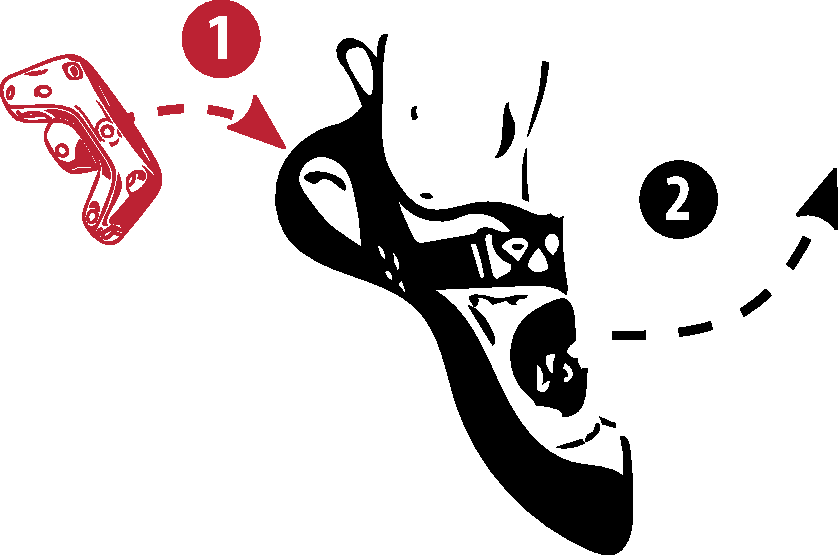
\includegraphics[scale=0.3]{include/images/climbing-shoe-with-instructions-on.pdf}
\end{textblock}
\pagebreak